% Machine translated from the Danish original, ../danish/ad-problems-2025-june.tex
\noindent\emph{This problem set has been machine translated from the Danish original.}
\medskip

\section*{Multiple-choice}\label{sec:mc}

\placeholder{Where to enter the multiple-choice answers, e.g.\ the multiple-choice module of the exam system.}

\multiplechoicestart

\question{Recurrences}
Assume that $T_i(n)=1$ for $n \leq 1$ for $i=1,\dots,6$. Which of the following statements about the solution to a recurrence are true?
\multipleanswers
\optionsstart
\answer $T_1(n) = 2\cdot T_1(n/2) + \Theta(n)$ has the solution $T_1(n) = \Theta(n \log n)$. \correct
\answer $T_2(n) = T_2(n/4) + \Theta(n)$ has the solution $T_2(n) = \Theta(n)$. \correct
\answer $T_3(n) = 3\cdot T_3(n/3) + \Theta(n \log n)$ has the solution $T_3(n) = \Theta(n \log^2 n)$. \correct
\answer $T_4(n) = 7\cdot T_4(n/2) + \Theta(n^2)$ has the solution $T_4(n) = \Theta(n^3)$.
\answer $T_5(n) = T_5(n-1) + \Theta(\log n)$ has the solution $T_5(n) = \Theta(\log^2 n)$.
\answer $T_6(n) = 4\cdot T_6(n/2) + \Theta(n \log n)$ has the solution $T_6(n) = \Theta(n^2)$. \correct
\optionsend

\explanation{
$T_1$: The master theorem with $a=2$, $b=2$, $f(n)=\Theta(n)$ gives $\Theta(n \log n)$.
$T_2$: $a=1$, $b=4$, $f(n)=\Theta(n) = \Omega(n^{\log_b a + \varepsilon})$, so the solution is $\Theta(n)$.
$T_3$: Master theorem case 2 (the borderline case), $a=3$, $b=3$, $f(n)=\Theta(n \log n)$ gives $\Theta(n \log^2 n)$.
$T_4$: $a=7$, $b=2$, $f(n)=\Theta(n^2)$; since $n^{\log_b a} = n^{\log_2 7}$ and $f(n)$ grows more slowly, the solution is $\Theta(n^{\log_2 7})$.
$T_5$: By induction one sees that the solution is the sum of $\log i$ for $i=1$ to $n$, which is $\Theta(n \log n)$, not $\log^2 n$.
$T_6$: $a=4$, $b=2$, $f(n)=\Theta(n \log n)$ and $n^{\log_b a} = n^2$; since $f(n) = o(n^2)$, case 1 of the master theorem applies and gives $\Theta(n^2)$.
}


\question{Merge-Sort variant}
Consider a variant of {\sc Merge-Sort} that splits the input into four parts, each of size roughly $n/4$, sorts them recursively, and merges the four sorted parts using three calls to {\sc Merge} (from CLRS Section 2.3). The pseudocode is:

{\small\begin{codebox}
  \Procname{$\proc{Merge4-Sort}(A, p, s)$}
  \li \If $p<s$ \Do
  \li $q_1 = \lfloor (3p+s)/4\rfloor$
  \li $q_2 = \lfloor (p+s)/2\rfloor$
  \li $q_3 = \lfloor (p+3s)/4\rfloor$
  \li $\proc{Merge4-Sort}(A, p, q_1)$
  \li $\proc{Merge4-Sort}(A, q_1+1, q_2)$
  \li $\proc{Merge4-Sort}(A, q_2+1, q_3)$
  \li $\proc{Merge4-Sort}(A, q_3+1, s)$
  \li $\proc{Merge}(A, p, q_1, q_2)$
  \li $\proc{Merge}(A, p, q_2, q_3)$
  \li $\proc{Merge}(A, p, q_3, s)$ \End
\end{codebox}}

\noindent
Which recurrence describes the running time $T(n)$ of $\proc{Merge4-Sort}$ on an input of size $n$ (where $n=s-p+1$)?
\oneanswer
\optionsstart
\answer $T(n) = 3\cdot T(n/4) + \Theta(n)$
\answer $T(n) = 3\cdot T(n/4) + \Theta(n\lg n)$
\answer $T(n) = 3\cdot T(n/4) + \Theta(n^2)$
\answer $T(n) = 4\cdot T(n/4) + \Theta(n)$ \correct
\answer $T(n) = 4\cdot T(n/4) + \Theta(n\lg n)$
\answer $T(n) = 4\cdot T(n/4) + \Theta(n^2)$
\optionsend
\explanation{The four recursive calls run on inputs of size approximately~$n/4$, and the remaining operations, including the three calls to {\sc Merge}, take $\Theta(n)$ time in total. Hence $T(n)=4\cdot T(n/4)+\Theta(n)$.}

\question{Stooge sort}
Consider this algorithm, which takes as input an array $A[1:n]$ and two indices $i,j$, where $i\leq j$.
It can be shown that $A$ is sorted by the call $\proc{Stooge-Sort}(A, 1, n)$.
\begin{codebox}
\Procname{$\proc{Stooge-Sort}(A, i, j)$}
\li \If $A[i] > A[j]$ \Then
\li     swap $A[i]$ with $A[j]$
    \End
\li \If $j \geq i + 2$ \Then
\li     $t = \lfloor (j - i + 1) / 3 \rfloor$
\li     $\proc{Stooge-Sort}(A, i, j - t)$
\li     $\proc{Stooge-Sort}(A, i + t, j)$
\li     $\proc{Stooge-Sort}(A, i, j - t)$
    \End
\end{codebox}
Let $T(n)$ be the running time of the call $\proc{Stooge-Sort}(A, 1, n)$, where $A$ is an array of length $n$.
Which of the following statements hold for $T(n)$?
\multipleanswers
\optionsstart
\answer The running time is described by the recurrence
\[
T(n) =
\begin{cases}
\Theta(1), & \text{for } n = 1 \\
3\,T(n-1) + \Theta(1), & \text{for } n > 1.
\end{cases}
\]
\itxanswer{T(n) = 3T(n-1) + Theta(1)}
\answer The running time is described by the recurrence
\[
T(n) =
\begin{cases}
\Theta(1), & \text{for } n = 1 \\
3\,T(n/3) + \Theta(1), & \text{for } n > 1.
\end{cases}
\]
\itxanswer{T(n) = 3T(n/3) + Theta(1)}
\answer The running time is described by the recurrence \correct
\[
T(n) =
\begin{cases}
\Theta(1), & \text{for } n = 1 \\
3\,T(2n/3) + \Theta(1), & \text{for } n > 1.
\end{cases}
\]
\itxanswer{T(n) = 3T(2n/3) + Theta(1)}
\answer The running time is $T(n)=\Theta(n^{\log_{3/2}3})$.\correct
\itxanswer{The running time is T(n)=Theta(n^{log_{3/2}(3)}).}
\answer The running time is $T(n)=\Theta(3^n)$.
\answer The running time is $T(n)=\Theta(n \log n)$.
\optionsend
\explanation{The algorithm is called recursively on three subarrays whose size is (up to rounding) two thirds of the original array.
Therefore the running time is given by \[
T(n) =
\begin{cases}
\Theta(1), & \text{for } n = 1 \\
3T(2n/3) + \Theta(1), & \text{for } n > 1,
\end{cases}
\]
which the master theorem solves as $T(n)=\Theta(n^{\log_{3/2}3})$.
}

\question{Kryptos}
Consider this algorithm, which takes as input an array $A[1:n]$ and indices $i,j$, where $i\leq j$.
\begin{codebox}
\Procname{$\proc{Kryptos}(A, i, j)$}
\li \If $i==j$ \Do
\li     \Return $-A[i]$
\End
\li $m=\lfloor\frac{i+j}2\rfloor$
\li \Return $\proc{Kryptos}(A, i, m)+\proc{Kryptos}(A, m+1,j)$
\end{codebox}
Which of the following statements about the call $\proc{Kryptos}(A, 1, n)$ are correct?
\multipleanswers
\optionsstart
\answer The running time is $\Theta(\log n)$.
\answer The running time is $\Theta(n)$.\correct
\answer The running time is $\Theta(n \log n)$.
\answer The running time is $\Theta(n^2)$.
\answer The algorithm returns $-\sum_{i=1}^n A[i]$.\correct
\answer The algorithm returns $\sum_{i=1}^n A[i]$.
\answer The algorithm returns $\sum_{i=1}^n (-1)^i A[i]$.
\optionsend
\explanation{The algorithm uses divide-and-conquer to sum the numbers in $A$, but with a negative sign because of the base case $i==j$.
The running time is described by the recurrence $T(n)=2T(n/2)+\Theta(1)$, which gives $T(n)=\Theta(n)$.
}


\question{Work and span}
Consider this parallel, recursive sorting algorithm:
%
\begin{codebox}
  \Procname{$\proc{Parallel-Merge-Sort}(A, p, r)$}
  \li \If $p<r$ \Do
  \li $q = \lfloor (p+r)/2\rfloor$
  \li \Spawn $\proc{Parallel-Merge-Sort}(A, p, q)$
  \li \Spawn $\proc{Parallel-Merge-Sort}(A, q+1, r)$
  \li     \Sync
  \li $\proc{Merge}(A, p, q, r)$ \End
\end{codebox}
Here $\proc{Merge}$ is the serial procedure for merging two sorted lists described in CLRS Chapter 2.
Now consider a call $\proc{Parallel-Merge-Sort}(A, 1, n)$ on an array of length $n$.
What are the \emph{work} and the \emph{span} of this call?
\oneanswer
\optionsstart
\answer Work $T_1=\Theta(\log n)$, span $T_\infty=\Theta(\log n)$
\answer Work $T_1=\Theta(\log n)$, span $T_\infty=\Theta(n)$
\answer Work $T_1=\Theta(n)$, span $T_\infty=\Theta(\log n)$
\answer Work $T_1=\Theta(n)$, span $T_\infty=\Theta(n)$
\answer Work $T_1=\Theta(n \log n)$, span $T_\infty=\Theta(\log n)$
\answer Work $T_1=\Theta(n \log n)$, span $T_\infty=\Theta(n)$\correct
\optionsend

\explanation{
The algorithm uses $\Theta(n \log n)$ work, just like ordinary merge sort.
Although the recursive calls run in parallel, $\proc{Merge}$ is called sequentially along the depth of the recursion and takes $\Theta(n)$ time at the top level.
This dominates the length of the critical path, since the input size is halved at each level of recursion: $\sum_{i=0}^{\log n} n/2^i < 2n$.
}


\question{Parallel algorithms}
Assume that a parallel algorithm on inputs of size $n$ has \emph{work} $T_1=\Theta(n^2)$ and \emph{span} $T_\infty=\Theta(\sqrt{n})$.
We are interested in the time $T_P$ needed to run the algorithm on $P$ processors with a \emph{greedy scheduler}.
Which of the statements below are correct?
\multipleanswers
\optionsstart
\answer If $P = \Theta(1)$ then $T_P = O(n^2)$ \correct
\answer If $P = \Theta(\log{n})$ then $T_P = O(n^{3/2})$
\itxanswer{If P = Theta(log n) then T_P = O(n^{3/2})}
\answer If $P = \Theta(\sqrt{n})$ then $T_P = O(n \log n)$
\answer If $P = \Theta(n)$ then $T_P = O(n)$ \correct
\answer If $P = \Theta(n^{3/2})$ then $T_P = O(\sqrt{n})$ \correct
\answer If $P = \Theta(n^2)$ then $T_P = O(1)$
\optionsend
\explanation{By CLRS Theorem 26.1, $T_P \leq T_1 / P + T_\infty$. Substituting the values of $P$ gives the following bounds: 1. $T_P = O(n^2)$, 2. $T_P = O(n^2/\log n)$, 3. $T_P = O(n^{3/2})$, 4. $T_P = O(n)$, 5. $T_P = O(\sqrt{n})$, 6. $T_P = O(\sqrt{n})$. These bounds match the statements in 1., 4., and 5., but are weaker than the bounds in 2., 3., and 6. By Theorem 26.2 these bounds are within a factor of 2 of optimal, so those statements cannot be true.
}

\question{Fibonacci heaps}
This problem concerns Fibonacci heaps as described in CLRS online Chapter 19.
The figure below shows a Fibonacci heap with both specified and unspecified nodes (the unspecified nodes are marked with question marks).
Which keys are possible for \emph{at least one} of the two nodes marked with a question mark?
\begin{center}
  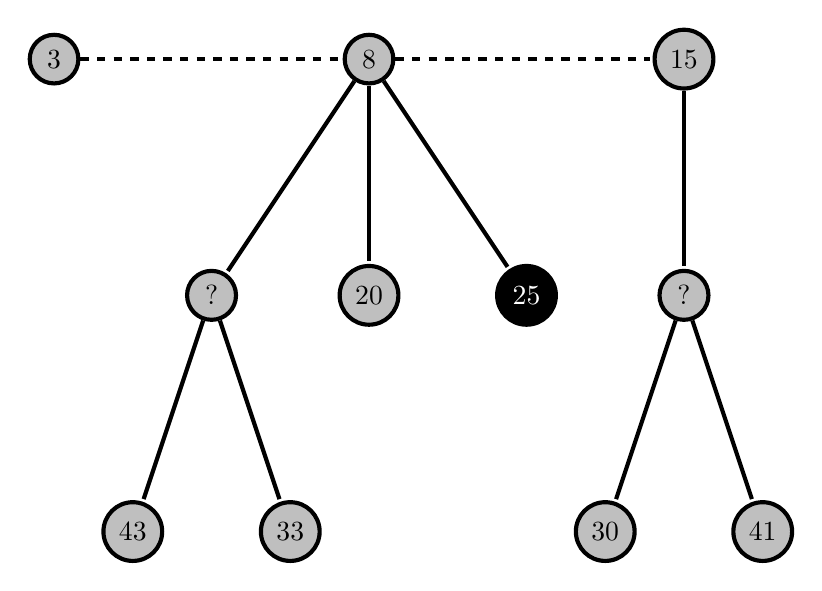
\begin{tikzpicture}[-,>=stealth,shorten >=1pt,auto,
      main node/.style={circle,draw}, line width=1.5pt]
  \node[main node,fill=lightgray] (a) at (-1,0) {3};
  \node[main node,fill=lightgray] (b) at (3,0) {8};
  \node[main node,fill=lightgray] (c) at (7,0) {15};
  \node[main node,fill=lightgray] (d) at (1,-3) {?};
  \node[main node,fill=lightgray] (e) at (3,-3) {20};
  \node[main node,fill=black,text=white] (f) at (5,-3) {25};
  \node[main node,fill=lightgray] (g) at (7,-3) {?};
  \node[main node,fill=lightgray] (h) at (2,-6) {33};
  \node[main node,fill=lightgray] (j) at (0,-6) {43};
  \node[main node,fill=lightgray] (i) at (6,-6) {30};
  \node[main node,fill=lightgray] (k) at (8,-6) {41};
  \path[every node/.style={font=\small}]
  (a) edge[dashed] (b)
  (b) edge[dashed] (c)
  (b) edge (d)
  (b) edge (e)
  (b) edge (f)
  (c) edge (g)
  (d) edge (h)
  (g) edge (i)
  (d) edge (j)
  (g) edge (k)
  ;
  \end{tikzpicture}
\end{center}
\multipleanswers
\optionsstart
\answer 3
\answer 5
\answer 12 \correct
\answer 18 \correct
\answer 32 \correct
\answer 42
\optionsend
\explanation{For the node on the left, the key must lie between 8 and 33 (the smallest key among its children), so 12, 18, and 32 are possible. For the node on the right, the key must lie between 15 and 30, which gives no further possibilities.}


\question{Longest common subsequence}
Which of these strings are longest common subsequences of the strings \texttt{AABCBDAA} and \texttt{BACDBAAB}?
\multipleanswers

\optionsstart
\answer \texttt{ABCBA}
\answer \texttt{ABCAB}
\answer \texttt{ACBAA}\correct
\answer \texttt{ACDAA}\correct
\answer \texttt{BBDAA}
\answer \texttt{BBCDA}
\answer \texttt{BCBAA}\correct
\answer \texttt{BCDAA}\correct
\optionsend

%Longest Common Subsequence returned by std. algo: ACBAA
%Alternative LCS: BCBAA, BCDAA, ACDAA

\explanation{Running the longest-common-subsequence algorithm from CLRS Section 15.4 by hand gives this dynamic programming table:
\begin{center}
\begin{tabular}{c|c|c|c|c|c|c|c|c|c||}
    &   & B & A & C & D & B & A & A & B\\
    \hline
     & 0 & 0 & 0 & 0 & 0 & 0 & 0 & 0 & 0\\
     \hline
    A & 0 & $\uparrow0$ & $\nwarrow1$ & $\leftarrow1$ & $\leftarrow1$ & $\leftarrow1$ & $\nwarrow1$ & $\nwarrow1$ & $\leftarrow1$ \\
    A & 0 & $\uparrow0$ & $\nwarrow1$ & $\uparrow1$ & $\uparrow1$ & $\uparrow1$ & $\nwarrow2$ & $\nwarrow2$ & $\leftarrow2$ \\
    B & 0 & $\nwarrow1$ & $\uparrow1^*$ & $\uparrow1$ & $\uparrow1$ & $\nwarrow2$ & $\uparrow2$ & $\uparrow2$ & $\nwarrow3$ \\
    C & 0 & $\uparrow1$ & $\uparrow1$ & $\nwarrow2$ & $\leftarrow2$ & $\uparrow2$ & $\uparrow2$ & $\uparrow2$ & $\uparrow3$ \\
    B & 0 & $\nwarrow1$ & $\uparrow1$ & $\uparrow2$ & $\uparrow2$ & $\nwarrow3$ & $\leftarrow3$ & $\leftarrow3$ & $\nwarrow3$ \\
    D & 0 & $\uparrow1$ & $\uparrow1$ & $\uparrow2$ & $\nwarrow3$ & $\uparrow3^*$ & $\uparrow3$ & $\uparrow3$ & $\uparrow3$ \\
    A & 0 & $\uparrow1$ & $\nwarrow2$ & $\uparrow2$ & $\uparrow3$ & $\uparrow3$ & $\nwarrow4$ & $\nwarrow4$ & $\leftarrow4$ \\
    A & 0 & $\uparrow1$ & $\nwarrow2$ & $\uparrow2$ & $\uparrow3$ & $\uparrow3$ & $\nwarrow4$ & $\nwarrow5$ & $\leftarrow5$ \\
    \hline
\end{tabular}
\end{center}
In two places (marked with $^*$) one can ``choose the direction'' in two ways, which gives four correct longest common subsequences of length 5.
The other options are not common subsequences.
}


\question{Dynamic programming}
We consider the longest-common-subsequence algorithm in CLRS Section 15.4.
Assume that after running it on two strings, the table $b$ looks as shown below.
What is the length of a longest common subsequence?
%X = "ABRAMS"
%Y = "RAMADAN"
\begin{center}
\begin{tabular}{|c|c|c|c|c|c|c|}
    \hline
    $\uparrow$ & $\nwarrow$ & $\leftarrow$ & $\nwarrow$ & $\leftarrow$ & $\nwarrow$ & $\leftarrow$ \\
    \hline
    $\uparrow$ & $\uparrow$ & $\uparrow$ & $\uparrow$ & $\uparrow$ & $\uparrow$ & $\uparrow$ \\
    \hline
    $\nwarrow$ & $\uparrow$ & $\uparrow$ & $\uparrow$ & $\uparrow$ & $\uparrow$ & $\uparrow$ \\
    \hline
    $\uparrow$ & $\nwarrow$ & $\leftarrow$ & $\nwarrow$ & $\leftarrow$ & $\nwarrow$ & $\leftarrow$ \\
    \hline
    $\uparrow$ & $\uparrow$ & $\nwarrow$ & $\leftarrow$ & $\leftarrow$ & $\leftarrow$ & $\leftarrow$ \\
    \hline
    $\uparrow$ & $\uparrow$ & $\uparrow$ & $\uparrow$ & $\uparrow$ & $\uparrow$ & $\uparrow$ \\
    \hline
\end{tabular}
\end{center}
\oneanswer
\optionsstart
\answer 1
\answer 2
\answer 3\correct
\answer 4
\answer 5
\answer 6
\optionsend
\explanation{A longest common subsequence can be found by following the arrows from the bottom right corner: $\uparrow$, $\leftarrow$, $\leftarrow$, $\leftarrow$, $\leftarrow$, $\nwarrow$, $\nwarrow$, $\nwarrow$.
The longest common subsequence corresponds to the three $\nwarrow$ arrows.}


\question{Search trees}
We consider a binary search tree that contains $n$ distinct keys, $x_1,\dots,x_n$, and has height~$h$.
What can be said with certainty (without knowing anything else about the tree) about the time to search for the keys $x_1,\dots,x_n$?
\multipleanswers
\optionsstart
\answer The time is $\Theta(\log n)$ for the worst key $x_i$.
\answer The time is $\Theta(h)$ for the worst key $x_i$. \correct
\answer The time is $\Theta(n)$  for the worst key $x_i$.
\answer The time is $O(\log n)$ on average over $x_1,\dots,x_n$.
\answer The time is $O(h)$ on average over $x_1,\dots,x_n$. \correct
\answer The time is $O(n)$ on average over $x_1,\dots,x_n$. \correct
\optionsend
\explanation{The time is $\Theta(h)$ in the worst case, where we search for a key $x_i$ at depth $h$.
This implies that the average time is $O(h)$.
Since the tree is not necessarily balanced, the height can be larger than $O(\log n)$ (also on average), so the time is not $O(\log n)$. Similarly, the height can be $o(n)$, so the time is not $\Omega(n)$. }


\question{Red-black search trees}
Consider a red-black binary search tree $T$, as described in CLRS Chapter 13, where the leaves are omitted and two internal nodes are unspecified:
\begin{center}
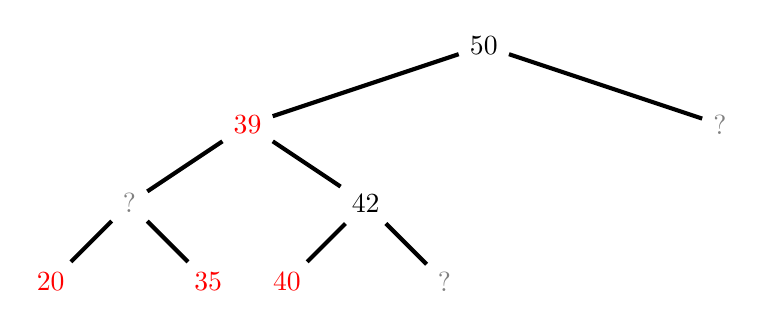
\begin{tikzpicture}[-,>=stealth,level/.style={sibling distance = 6cm/#1,
    level distance = 1cm}, line width=1.5pt]
  \node [black] {50}
      child{ node [red] {39}
              child{ node [gray] {?}
                  child{ node [red] {20} }
                  child{ node [red] {35}}
              }
              child{ node [black] {42}
                              child{ node [red] {40}}
                              child{ node [gray] {?}}
              }
      }
      child{ node [gray] {?}
          }
  ;
  \end{tikzpicture}
\end{center}
\noindent
Which nodes are possible for \emph{at least one} of the three unspecified positions if the tree must satisfy the red-black properties?
\multipleanswers
\optionsstart
\answer A red node with key 25.
\answer A black node with key 32. \correct
\answer A black node with key 38.
\answer A red node with key 45. \correct
\answer A black node with key 55. \correct
\answer A red node with key 60.
\answer A black node with key 70. \correct
\optionsend
\explanation{ Every path from the root to a leaf must contain the same number of black nodes, i.e.,~there must be two on every path. This means that the nodes, from left to right, have the colors black, red, black. Moreover, the keys must be placed so that the binary-search-tree property is maintained.}


\question{Minimum spanning tree}
Consider this weighted graph:
\begin{center}
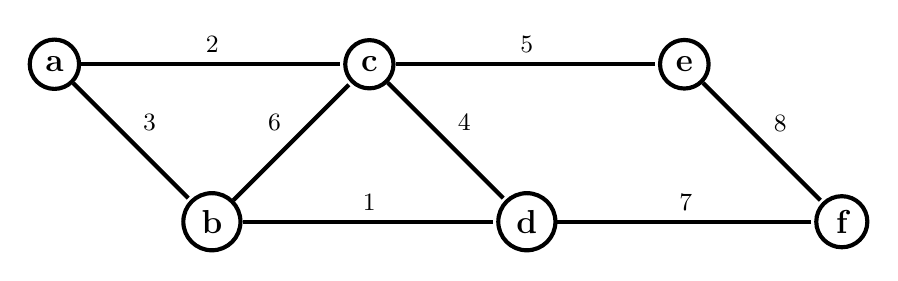
\begin{tikzpicture}[-,>=stealth,shorten >=1pt,auto,
  main node/.style={circle,draw,font=\large\bfseries}, line width=1.5pt]
\node[main node] (a) at (0,2) {a};
\node[main node] (b) at (2,0) {b};
\node[main node] (c) at (4,2) {c};
\node[main node] (d) at (6,0) {d};
\node[main node] (e) at (8,2) {e};
\node[main node] (f) at (10,0) {f};

\path[every node/.style={font=\small}]
(a) edge node {3} (b)
(a) edge node {2} (c)
(b) edge node {1} (d)
(c) edge node {4} (d)
(c) edge node {5} (e)
(d) edge node {7} (f)
(e) edge node {8} (f)
(b) edge node {6} (c);
\end{tikzpicture}
\end{center}
The minimum spanning tree is unique. Which edges belong to the minimum spanning tree?
\multipleanswers
\optionsstart
\answer \{a,b\} \correct
\answer \{a,c\} \correct
\answer \{b,c\}
\answer \{b,d\} \correct
\answer \{c,d\}
\answer \{c,e\} \correct
\answer \{d,f\} \correct
\answer \{e,f\}
\optionsend
\explanation{Applying, e.g., Prim's algorithm shows that the marked edges belong to the MST.}

\question{Minimum spanning tree}
Consider a weighted, undirected graph with vertex set $V = \{1,2,\ldots,n\}$ and edges between all pairs of vertices.
The edge from vertex $u$ to vertex $v$ has weight $w(u,v) = |u-v|$.
The graph for the case $n=4$ is shown below.

\begin{center}
  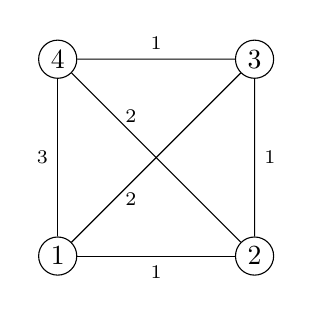
\begin{tikzpicture}[scale=1.25,
    vertex/.style={circle, draw, fill=white, inner sep=2pt},
    every edge/.style={draw}]
  % Define positions of vertices
  \node[vertex] (1) at (0,0) {1};
  \node[vertex] (2) at (2,0) {2};
  \node[vertex] (3) at (2,2) {3};
  \node[vertex] (4) at (0,2) {4};
  % Draw edges with weights (no circles on weights)
  \draw (1) -- (2) node[midway, below] {\scriptsize $1$};
  \draw (1) -- (3) node[pos=0.35, below] {\scriptsize $2$};
  \draw (1) -- (4) node[midway, left] {\scriptsize $3$};
  \draw (2) -- (3) node[midway, right] {\scriptsize $1$};
  \draw (4) -- (2) node[pos=0.35, above] {\scriptsize $2$};
  \draw (3) -- (4) node[midway, above] {\scriptsize $1$};
\end{tikzpicture}
\end{center}

What is the weight of the minimum spanning tree, as a function of $n$?
\oneanswer
\optionsstart
\answer $\Theta(\sqrt{n})$
\answer $\Theta(n)$ \correct
\answer $\Theta(n \log n)$
\answer $\Theta(n^2)$
\answer $\Theta(2^n)$
\optionsend

\explanation{
To find a minimum spanning tree (MST) we must choose $n-1$ edges such that all $n$ vertices are connected without forming a cycle and the sum of the weights is as small as possible.
One strategy is to connect the vertices in order: $1$ with $2$, $2$ with $3$, etc., i.e., use the edges $\{1,2\}$, $\{2,3\}$, $\{3,4\}$, ..., $\{n-1,n\}$. Each of these edges has weight $1$, and there are $n-1$ of them, so the total weight is $M_n = n-1$.
Since no weight is smaller than 1, this is optimal.
Hence the weight of the MST grows as $\Theta(n)$.%, since the weight grows linearly with $n$.
}
%For an integer $n >0$, let $K_n = (V_n,E_n)$ be the complete graph on the vertex-set $V = \{1,2,\ldots,n\}$. Let $W_n : E_n \to \mathbb{R}$
%be defined by
%$W_n(e) = |i-j|$ where $e = \{i,j\} \in E_n$.
%Denote by $M_n$ the weight of a minimum spanning tree for $K_n$ with respect to $W_n$.
%Which of the following is true?
%\optionsstart
%\answer $M_n = \Theta(n)$ \correct
%\answer $M_n = \Theta(n^2)$
%\answer $M_n = \Theta(\sqrt{n})$
%\answer $M_n = \Theta(2^n)$
%\answer $M_n = \Theta(n \log n)$
%\optionsend


\question{Shortest paths}
Consider a weighted, directed graph with vertex set $V = \{1,2,\ldots,n\}$ and one edge between every pair of vertices.
For vertices $u$ and $v$ with $u<v$ there is an edge from $u$ to $v$ with weight $w(u,v) = v$, but no edge from $v$ to $u$.
The graph for the case $n=5$ is shown below.
%Fix an integer $n >0$,
%and consider the set of vertices $V = \{1,2,\ldots,n\}$.
%For all distinct $i,j \in V$,
%define the weight of the directed edge $e = (i,j)$ as $W(e) = j$.
%There is no edge $(j,i)$ when $j>i$.
%Below, as an example, is the graph for $n=5$.
%
\begin{center}
\begin{tikzpicture}[
    >=Stealth,
    vertex/.style={circle, draw, minimum size=1cm},
    edge/.style={->, thick}
  ]
  % Nodes
  \node[vertex] (1) at (0,0) {1};
  \node[vertex] (2) at (2,1.5) {2};
  \node[vertex] (3) at (4,0) {3};
  \node[vertex] (4) at (6,1.5) {4};
  \node[vertex] (5) at (8,0) {5};

  % Edges with straight lines
  \draw[edge] (1) -- node[midway, sloped, above] {2} (2);
  \draw[edge] (1) -- node[midway, sloped, below] {3} (3);
  \draw[edge] (1) to[bend right=30] node[midway, below] {5} (5); % curved
  \draw[edge] (1) to[bend left=55] node[midway, above] {4} (4); % curved

  \draw[edge] (2) to[bend right=15] node[midway, above] {3} (3); % curved
  \draw[edge] (2) -- node[midway, sloped, above] {4} (4);
  \draw[edge] (2) to[bend left=55] node[midway, above] {5} (5); % curved

  \draw[edge] (3) to[bend right=15] node[midway, above] {4} (4); % curved
  \draw[edge] (3) -- node[midway, sloped, below] {5} (5);

  \draw[edge] (4) -- node[midway, sloped, above] {5} (5);

\end{tikzpicture}
\end{center}
%
Let $\delta(u,v)$ denote the length of a shortest path in the graph from $u$ to $v$.
What is the largest distance from vertex $1$ to another vertex in the graph, i.e.,~what is $\max_v(\delta(1,v))$?
\oneanswer
%Fix an integer $n >0$,
%and consider the vertex-set $V = \{1,2,\ldots,n\}$.
%For every distinct $i,j \in V$,
%define the weight of the directed edge $e = (i,j)$ by $W(e) = j^2$.
%Denote by $D(i,j)$ the shortest path distance with respect to $W$ between $i$ and $j$.
%What is the maximum distance from the vertex $1$?
\optionsstart
\answer $\lceil n/2\rceil$
\itxanswer{ceiling(n/2)}
\answer $n$ \correct
\answer $\lceil 3n/2\rceil$
\itxanswer{ceiling(3n/2)}
\answer $2n$
\optionsend

\explanation{The shortest path from $1$ to $j$ is always the direct edge, which can be shown by induction on $n$. That is,~$\delta(1,j) = j$, which is at most $n$. Alternatively, all other options can be ruled out by looking at the example above.}


\question{Bellman-Ford}
Consider the directed graph $G$ below, with an unspecified weight $x$:
\begin{center}
\begin{tikzpicture}[
    >=Stealth,
    vertex/.style={circle, draw, minimum size=1cm},
    edge/.style={->, thick}
  ]
  % Nodes
  \node[vertex] (1) at (0,0) {1};
  \node[vertex] (2) at (2,1.5) {2};
  \node[vertex] (3) at (4,0) {3};
  \node[vertex] (4) at (6,1.5) {4};
  \node[vertex] (5) at (8,0) {5};

  % Edges with straight lines
  \draw[edge] (1) -- node[midway, sloped, above] {-1} (2);
  \draw[edge] (3) -- node[midway, sloped, below] {4} (1);
  \draw[edge] (1) to[bend right=25] node[midway, below] {6} (5); % curved

  \draw[edge] (2) to[bend right=0, sloped] node[midway, above] {$x$} (3); % curved
  \draw[edge] (4) -- node[midway, sloped, above] {2} (2);

  \draw[edge] (3) to[bend right=0, sloped] node[midway, above] {-3} (4); % curved
  \draw[edge] (3) -- node[midway, sloped, below] {0} (5);

  \draw[edge] (5) -- node[midway, sloped, above] {3} (4);

\end{tikzpicture}
\end{center}

Let $w_x$ denote the weight vector of $G$.
For which values of $x$ does $\proc{Bellman-Ford}(G, w_x, 1)$ from CLRS Section 22.1 return {\sc True}?
\multipleanswers
\optionsstart
\answer $x=2$\correct
\answer $x=1$\correct
\answer $x=0$
\answer $x=-1$
\answer $x=-2$
\optionsend
\explanation{If $x\leq 0$ there is a negative cycle through vertices 2, 3, 4 that is reachable from vertex~1, so $\proc{Bellman-Ford}$ returns {\sc False}. If $x\geq 1$ there is no negative cycle in the graph, so $\proc{Bellman-Ford}$ returns {\sc True}.}


\question{Choice of algorithm}
Given two unsorted arrays $A[1:n]$ and $B[1:m]$ with $n$ and $m$ elements, respectively, we want to find the number of elements that occur in both arrays.
Neither array contains repeated elements, i.e.,~they contain $n$ and $m$ distinct elements, respectively.
Let $T$ be a red-black search tree. We consider two possible algorithms:
\begin{codebox}
\Procname{$\proc{Intersection-BruteForce}(A, B, n, m)$}
\li $count \gets 0$
\li \For $i \gets 1$ \To $n$
\li \Do
        \For $j \gets 1$ \To $m$
\li     \Do
            \If $A[i] = B[j]$
\li         \Then $count \gets count + 1$
            \End
        \End
    \End
\li \Return $count$
\end{codebox}
\begin{codebox}
\Procname{$\proc{Intersection-Tree}(A, B, n, m)$}
\li $T.root \gets \proc{nil}$ \Comment{$T$ is now an empty search tree}
\li \For $j \gets 1$ \To $m$
\li \Do \text{Let $z$ be a new, empty RB-tree node}
\li $z.key \gets B[j]$
\li $\proc{RB-Insert}(T, z)$ \End
\li $count \gets 0$
\li \For $i \gets 1$ \To $n$
\li \Do
        \If $\proc{Tree-Search}(T, A[i]) \neq \proc{nil}$
\li     \Then $count \gets count + 1$
     \End
    \End
\li \Return $count$
\end{codebox}
Which algorithm is asymptotically faster depends on the relationship between the parameters $m$ and $n$.
For which of the choices of $m$ below is $\proc{Intersection-BruteForce}$ asymptotically at least as fast as $\proc{Intersection-Tree}$?
\multipleanswers
\optionsstart
\answer $m = \Theta(1)$\correct
\answer $m = \Theta(n)$
\answer $m = \Theta(n^2)$
\answer $m = \Theta(2^n)$\correct
\optionsend
\explanation{The running time of $\proc{Intersection-BruteForce}$ is $\Theta(nm)$, while the running time of the procedure $\proc{Intersection-Tree}$ is $\Theta(m\log m + n\log m)$.
Substituting the four choices of $m$ into these running times gives: 1.~$\Theta(n)$ for both algorithms, 2.~$\Theta(n^2)$ and $\Theta(n\log n)$, respectively, 3.~$\Theta(n^3)$ and $\Theta(n^2\log n)$, respectively, 4.~$\Theta(n\cdot 2^n)$ for both algorithms.
}

\question{Matrix-chain multiplication}
The algorithm {\sc Matrix-Chain-Order}$(p,n)$ from CLRS 14.2 returns two arrays $m$ and $s$.
Below is an array $s[1:n-1, 2:n]$ returned by {\sc Matrix-Chain-Order}$(p,n)$ for a product of $n=6$ matrices $A_1\cdots A_6$ with dimensions given in $p$.
\medskip

\begin{tabular}{c|ccccc}
$i \backslash j$ & 2 & 3 & 4 & 5 & 6 \\
\hline
1 & 1 & 1 & 3 & 4 & 4 \\
2 &   & 2 & 3 & 4 & 4 \\
3 &   &   & 3 & 4 & 4 \\
4 &   &   &   & 4 & 5 \\
5 &   &   &   &   & 5 \\
\end{tabular}

\medskip\noindent
Give the parenthesization according to the table.
\oneanswer
%
\optionsstart
\answer $((A_1( A_2A_3))A_4)(A_5A_6)$.\correct
\answer $(A_1(A_2 A_3))((A_4 A_5)A_6)$
\answer $A_1((A_2(A_3A_4))(A_5 A_6))$
\answer $((((A_1 A_2)A_3)A_4)A_5)A_6$.
\answer $(A_1(A_2 A_3))(A_4(A_5 A_6))$.
\optionsend
\explanation{We run the algorithm {\sc Print-Optimal-Parens}$(s,1,n)$ by hand. Since $s[1,6]=4$, the outermost parentheses are $(A_1A_2A_3A_4)(A_5A_6)$.
This matches only option 1.}


\question{Disjoint sets}
We consider tree representations of \emph{disjoint sets}, as described in CLRS Section 19.3, using the \emph{union by rank} heuristic without path compression.
An algorithm makes $n$ calls to {\sc Make-Set}, $n^2$ calls to {\sc Find-Set}, and $n-1$ calls to {\sc Union}.
Which is the best (smallest) of the following time bounds that we can guarantee for the total time taken by these operations?
\oneanswer
\optionsstart
\answer The time is $O(n)$
\answer The time is $O(n \log n)$
\answer The time is $O(n^2)$
\answer The time is $O(n^2 \log n)$ \correct
\answer The time is $O(n^3)$
\answer The time is $O(n^3 \log n)$
\optionsend
\explanation{ The time is dominated by the $n^2$ {\sc Find-Set} operations, each of which has a time bound of $O(\log n)$.}


\multiplechoiceend

\newpage

\section*{Written problems}\label{sec:written}

% Machine translated from the Danish original, ../danish/skriftlige.tex
{\bf Written problems:} \placeholder{How the answers are submitted, e.g.\ the file format and exam system, and whether drawings made on a tablet may be inserted.}
\begin{itemize}
    \item Use \emph{one page for each subquestion, in the same order as in the problem set.}
    \item The number/letter of the subquestion (e.g.\ 19 or 20.a) must be stated.
\end{itemize}



\section{Splicing ropes (9\%)}

We consider a multiset $A$ of positive integers, which represent the lengths of the ropes we have available.
We can splice two ropes together, and the cost of doing so is the sum of their lengths.
That is, we can choose two numbers $x,y\in A$.
To \emph{splice} $x$ and $y$ means that we update $A$ to $(A\setminus\{x,y\})\cup\{x+y\}$.
The cost of this is $x+y$.
Note that $A$ is a multiset, which means that $A$ may contain several elements with the same value, and when we remove $x$, we remove only one element with value $x$ (and similarly for $y$).
We want to splice until $A$ contains only one value, such that the total cost is as small as possible.
We represent $A$ by an array.

\medskip

\textbf{Example:}
$A=\langle 3,1,7,2\rangle$.
We splice $1$ and $2$ at cost $3$ and get $A=\langle 3,7,3\rangle$.
We splice $3$ and $7$ at cost $10$ and get $A=\langle 3,10\rangle$.
We splice $3$ and $10$ at cost $13$ and get $A=\langle 13\rangle$.
The total cost of this splicing sequence is $3+10+13=26$.
Note that this splicing sequence is \emph{not} optimal, since it is possible to achieve a total cost of less than $26$.

\subquestion{a)}
{
Give the optimal splicing sequence and the total cost for $A=\langle 3,1,7,2\rangle$. You do not need to prove that the sequence is optimal.
}

\explanation{We splice $1,2$, then $3,3$, then $6,7$, and get a total cost of $3+6+13=22$.}

\subquestion{b)}
{
Describe an efficient algorithm that computes the smallest possible total cost of splicing until $A$ contains only one value.
}

\explanation{
We use a greedy algorithm that always splices the two smallest values in~$A$.
This gives the smallest possible total cost, by an argument similar to the proof of optimality of Huffman codes.
}

\subquestion{c)}
{
Explain how the algorithm from part b), or an improved algorithm, can be implemented so that the running time is $O(n\log n)$, where $n$ is the initial size of $A$.
}

\explanation{
We represent $A$ as a min-heap, so that we can extract the smallest elements and insert new elements in $O(\log n)$ time.
The total running time is then $O(n\log n)$, since we are done after splicing $n-1$ times.
}

\newpage
\section{Long paths in trees (11\%)}%\label{sec:last}

Consider a binary tree $T$ in which every node has either two children or none.
Let the root be $r$, and for every node $v$, let $v.left$ and $v.right$ be pointers to the left and right child, respectively.
If $v$ has no children, then $v.left=v.right=NIL$.
In this problem we look at lengths of paths in a tree -- for example, the tree below has a path of length 3 from the root $r$ to the leaf $y$ and a path of length 5 from the leaf $z$ to the leaf $w$.
%
\begin{center}
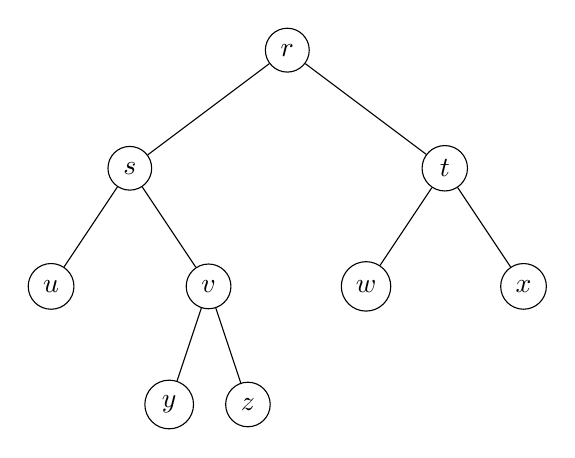
\begin{tikzpicture}[every node/.style={circle, draw},
  level distance=1.5cm,
  level 1/.style={sibling distance=4cm},
  level 2/.style={sibling distance=2cm},
  level 3/.style={sibling distance=1cm}]
\node {$r$}
  child {node {$s$}
    child {node {$u$}
    }
    child {node {$v$}
      child {node {$y$}}
      child {node {$z$}}
    }
  }
  child {node {$t$}
    child {node {$w$}}
    child {node {$x$}}
  };
\end{tikzpicture}
\end{center}


\subquestion{a)}
{We want to find the maximum length of a path from $r$ to a leaf.
The length of a path is the number of edges on the path.
Describe an algorithm that solves the problem.
The input to the algorithm is the root $r$.
You may write pseudocode, but a clear and precise description in words is also sufficient.
To get full points, the running time must be $O(n)$, where $n$ is the number of nodes in $T$.}

\explanation{We can solve the problem recursively by computing, for each node $v$, the longest path from $v$ to a leaf in the subtree rooted at $v$.
If $v.left==NIL$ we return $0$, since $v$ itself is a leaf.
Otherwise we solve the problem for both children and return the maximum of these plus $1$.
Here is the pseudocode, which we call with $v=r$:

\begin{codebox}
\Procname{$\proc{LongestPathToLeaf}(v)$}
\li \If $v.left==NIL$
\li \Then \Return $0$
\End
\li \Return $1+\max\{\proc{LongestPathToLeaf}(v.left),\proc{LongestPathToLeaf}(v.right)\}$
\end{codebox}
}

\subquestion{b)}
{The diameter of $T$ is the maximum length of a path in $T$.
Prove or disprove that a path of maximum length always starts and ends at leaves.}

\explanation{If a path starts or ends at a node that is not a leaf, the path can be extended to one of its children, since every node that is not a leaf has two children.
Therefore the longest path must both start and end at leaves.}

\subquestion{c)}
{Describe an algorithm that computes the diameter of $T$ and argue for its correctness.
The input to the algorithm is the root~$r$.
You may write pseudocode, but a clear and precise description in words is also sufficient.
To get full points, the running time must be $O(n)$, where $n$ is the number of nodes in $T$.}

\explanation{We first compute, in each node $v$, the value $v.h$, which is the length of the longest path from $v$ to a leaf below $v$, as in question a).
Let $v.s$ be the length of the longest path in the subtree rooted at $v$.
If $v.left=NIL$ we set $v.s=0$.
Otherwise there are two cases: either the longest path is contained in one of the subtrees rooted at one of the children, or it passes through $v$.
If it passes through $v$, then on the left side it must go down to a leaf that is deepest below $v.left$, and on the right side down to a leaf that is deepest below $v.right$.
Therefore we can compute $v.s$ as
\[
v.s=\max\{v.left.s,v.right.s,v.left.h+v.right.h+2\}.
\]
This can be written in pseudocode as follows, where we assume that the values $v.h$ have already been computed:

\begin{codebox}
\Procname{$\proc{LongestPathInTree}(r)$}
\li \If $r.left==NIL$
\li \Then \Return $0$
\End
\li $ls=\proc{LongestPathInTree}(r.left)$
\li $rs=\proc{LongestPathInTree}(r.right)$
\li \Return $\max\{ls,rs,r.left.h+r.right.h+2\}$
\end{codebox}
}

\newpage
\section{Minimum spanning tree (8\%)}\label{sec:last}

Let $(x_1,y_1),\ldots,(x_n,y_n) \in \mathbb{R}^2$ be (distinct) points in the plane.
Let $G = (V,E)$ denote the complete, undirected graph on the vertices $V = \{1,2,\ldots,n\}$.
Define the weight function $W : E \to \mathbb{R}$ as
$$W(\{i,j\}) = \sqrt{(x_i-x_j)^2+(y_i-y_j)^2},$$
i.e.,~the weight of the edge $\{i,j\}$ is the Euclidean distance between the points $(x_i,y_i)$ and $(x_j,y_j)$.
The drawing below illustrates a graph $G$ defined by 5 numbered points placed on a grid where each square has side length~1.

\begin{center}
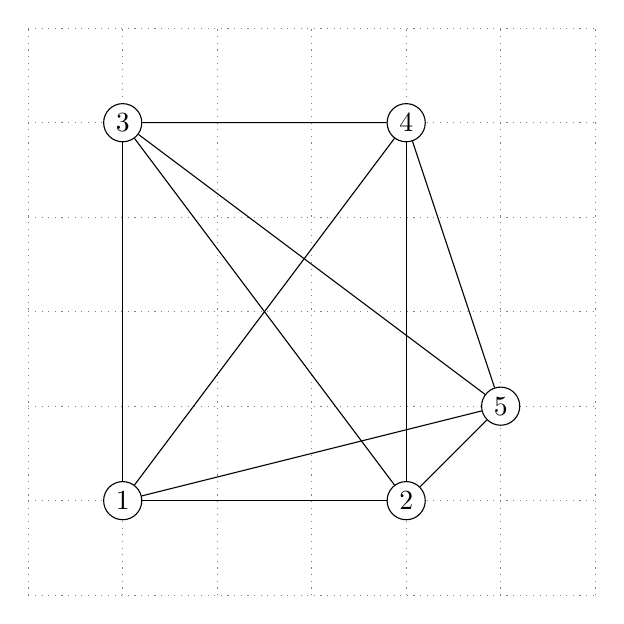
\begin{tikzpicture}[scale=1.2,
    vertex/.style={circle, draw, fill=white, inner sep=2pt},
    every edge/.style={draw}]

  % Draw background grid
  \draw[step=1,dotted,gray] (-1,-1) grid (5,5);

  % Define nodes at integer positions with known integer distances
  \node[vertex] (A) at (0,0) {1};
  \node[vertex] (B) at (3,0) {2};
  \node[vertex] (C) at (0,4) {3};
  \node[vertex] (D) at (3,4) {4};
  \node[vertex] (E) at (4,1) {5};

  % Draw all edges of the complete graph (10 edges)
  \draw (A) -- (B);
  \draw (A) -- (C);
  \draw (A) -- (D);
  \draw (A) -- (E);

  \draw (B) -- (C);
  \draw (B) -- (D);
  \draw (B) -- (E);

  \draw (C) -- (D);
  \draw (C) -- (E);

  \draw (D) -- (E);

\end{tikzpicture}
\end{center}

\subquestion{a)}
{Which edges form a minimum spanning tree for the graph $G$ illustrated above, and what is the total weight of these edges? A correct answer gives full points, but you are welcome to justify your answer.}

\explanation{The minimum spanning tree consists of the edges of the path 1--2--5--4--3. This can be confirmed by considering, for each edge of the path, the cut that splits the graph at that edge. The edge lengths are 3, $\sqrt{2}$, $\sqrt{10}$, 3, i.e.,~a total of $6+\sqrt{2}+\sqrt{10}\approx 10.5765$.\medskip}

Now consider an arbitrary graph $G$ with distances defined by a weight function $W$ as described above.
Let $F \subset E$ be the $n-1$ edges of a minimum spanning tree. We want to argue that there cannot be a pair of edges in $F$ that ``cross each other'' when the graph is drawn in the plane.
More specifically, for an edge $e = \{i,j\} \in E$, let $I_e$ denote the open line segment connecting the point $(x_i,y_i)$ and the point $(x_j,y_j)$:
$$I_e = \{ \lambda (x_i,y_i)+(1-\lambda) (x_j,y_j) : 0 < \lambda < 1\}.$$

\subquestion{b)}
{Prove that $F$ cannot have lines that cross each other. More specifically, show that for every choice of two edges $e,e' \in F$ we have $I_e \cap I_{e'} = \emptyset$.}

\explanation{
Assume for contradiction that there are two edges $e = \{a,b\}$ and $e' = \{c,d\}$ in $F$ that cross each other in their interiors, i.e.,~$I_e \cap I_{e'} \neq \emptyset$.
We claim that the edges can be replaced either by the edges $\{a,c\}$ and $\{b,d\}$ or by the edges $\{a,d\}$ and $\{b,c\}$ without introducing cycles.
This can be seen by considering all the ways in which $a$, $b$, $c$, $d$ can be connected in a tree structure.
By the triangle inequality this gives a new spanning tree with smaller total weight, which contradicts the assumption that $F$ is a minimum spanning tree.
}

%Let $n > 0$ be an integer and let $(x_1,y_1),\ldots,(x_n,y_n) \in \mathbb{R}^2$ be $n$ distinct points in the plane. Denote by $G = (V,E)$ the complete graph on the vertex-set $V = \{1,2,\ldots,n\}$. Define the weight function $W : E \to \mathbb{R}$ by
%$$W(e) = \sqrt{(x_i-x_j)^2+(y_i-y_j)^2}$$
%where $e = \{i,j\} \in E$.
%Fix a minimum spanning tree of $G$ with respect to $W$ and denote by $F \subset E$ the $n-1$ edges in it.
%For an edge $e = \{i,j\} \in E$,
%denote by $I_e$ the open line segment connecting the point $(x_i,y_i)$
%and the point $(x_j,y_j)$:
%$$I_e = \{ \lambda (x_i,y_i)+(1-\lambda) (x_j,y_j) : 0 < \lambda < 1\}.$$
%Prove that for every two distinct edges $e,e' \in F$,
%the intersection $I_e \cap I_{e'}$
%is empty.

%Sketch: If there is a crossing, there are two ways to flip the edges. Both ways lead to lower total weight by the triangle inequality. One of the two ways does not create cycles.



\label{page:last}
